\title{Engineering inclusivity in online conversations: a preliminary note}
\author{Alberto Cottica}
\date{July 2016}

\documentclass{article}
\usepackage{graphicx}
\usepackage{subcaption}
\usepackage{mathtools}
\usepackage{csquotes}
\graphicspath{ {./Paper3Images/} }
\usepackage{hyperref}
\usepackage{enumitem}

\setlength{\parindent}{0em}
\setlength{\parskip}{1em}

\begin{document}

\maketitle

\begin{abstract}

	In their paper "Group Intimacy and Network Formation" (\cite{kim2015group}), Kim, Jo and Kim observe that some online communities display a bizarre behaviour: they are open to new entrants, yet new entrants can never quite become full participants in the way that the founders are. They try to account for this by building a simulation model. This is intriguing in terms of the thesis, because the inclusivity towards new entrants is a key concern of real-world online communities. 

	We propose to extend and improve on their results in three ways. First, we consider the same issue from the perspective of the entity (company or public sector agency) which created the online community. Inclusivity maps to user engagement and community growth, which is seen as desirable in most real-life cases. We consider the decision to enact community management policies to this effect. Second, we alter the specification of the model. The new specification accounts for the observed fact that each user's behaviour is dependent on the behaviour of other users in ways that account for the "bursty" nature of human communication. We explore whether Kim, Jo and Kim's result is robust to the new specification. Third, we introduce community managers in the model, and test whether they have an impact on the results, making the online community more inclusive and less "founders-dominated".

\end{abstract}

\section{Main engine of the model}

We model an online community that supports person-to-person communication. Every member of the community has technological affordances and social permission to communicate with any other member. Members prefer to communicate with people they are more familiar ("intimate", in the language of Kim, Jo and Kim) with. Familiarity is built via communication events. Familiarity is time-discounted: older communication events have a weaker effect on present familiarity than more recent ones. The online community is assumed to grow over time. 

Communication events crystallise into an intimacy network, which is directed and weighted. The sum of the weights of the incoming edges in this network encodes "membership strength", deonted by $S_i$. The distribution of membership strength is Kim, Jo and Kim's way to measure inclusivity in an online community. In "cliquish", exclusionary communities, members prefer to interact only with their close circle of friends. As a result, many members have low membership strength. In their model, this results in leaving the community altogether. Inclusive communities are characterised by a more equal distribution of membership strength. 

The model consists of the following five phases:

\begin{enumerate}
	\item Initialization.
	\item New members join the community.
	\item Each member decides \textit{whether} to engage in communication.
	\item Each member that has decided to engage in communication decides \textit{with whom} to communicate.
	\item The intimacy network is updated.
\end{enumerate}

Phases 2-5 are iterated multiple times. The model's results consist in the evolution path and end state of the community's intimacy network \footnote{Chapters 1 and 2 in the thesis focus on the \textit{interaction} network instead.}.

\section{Initialization}

We start with two members, mutually connected in the intimacy network. Let $W(t_0)_{i,j}$ be the intimacy felt by person $i$ for person $j$ at time $t_0$ (and note that $W_{i,j} \neq W_{j,i}$):

\begin{equation}
	W(t_0)_{i,j} = W(t_0)_{j,i} > 0	
\end{equation}

\subsection{More on initialisation}

Our approach to initialisation is grounded in the literature on evolving networks (for example \cite{barabasi1999emergence}) and in empirical observation of real-life online communities. For an example of the latter, see Figure \ref{fig:growthER}. 

\begin{figure}
	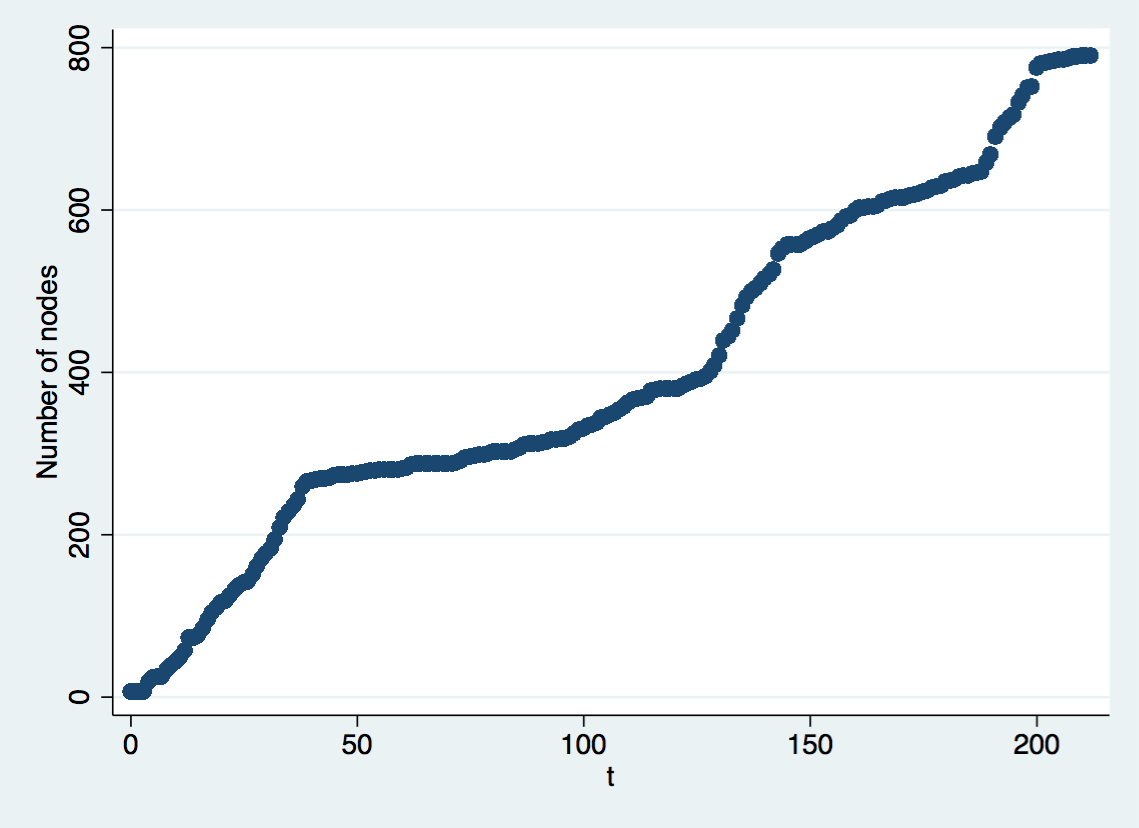
\includegraphics[width = \textwidth]{Growth_ER} 
	\caption{Number of user accounts in Edgeryders from inception to four years after}
	\label{fig:growthER}
\end{figure}

Kim, Jo and Kim take a very different approach to initialisation. They start with a network of 150 members, all connected to each other. All edges have strength 0.1. This means that all "founders" have incoming intimacy of $149 \times 0.1 = 14.9$ at the start. Each simulation runs for 800 time steps; a new member is added every four time steps, so that network size at $t = 800$ is 350. 

For high values of the intimacy parameter $\beta$ (see below), they find that the community splits almost exactly into two: all but about 20 of the "founders" are still connected, and some have achieved "dominance". The great majority of nodes added afterwards have removed themselves from the network . About 30 are still active. None that joined after $t = 100$ has achieved "dominance" (figure 2c in their paper). There is the possibility that the peculiar initialisation (a 150-clique, almost never observed in the real world) exacerbates the dynamics excluding new users, because the founders already have many people to talk to. 

\section{Network growth}

At each time step, $\alpha$ new members join the community. This is consistent with the literature on evolving networks and with \cite{kim2015group}.

\section{Deciding whether to engage}

Not all members engage in communication with other members at each time period. Again, this is consistent with observation of real-life online communities: in Edgeryders, the number of communication events that users (other than community managers) engaged in at each one-week time period was typically zero (no communication occurred in 98.92\% of observations, $N = 82,297$). Previous work (\cite{cottica2016microfoundations}) has found that to depend on incoming communications, so we model it as follows:

\begin{equation}
	P[comm_i(t_n) = 1] = \Theta [C, \phi_{j,i}(t_{n-1})], \forall j \neq i
	\label{eq:engageYesNo}
\end{equation}

Where:

\begin{itemize}
	\item $\Theta$ is a function whose codomain is the interval $[0,1]$.
	\item $C$ is a constant. It can  be thought of as a "chattiness" parameter: the higher its value, the higher the probability that users will engage in communication, all other things being equal.
	\item  $\phi_{j,i}(t_{n-1})$ indicates the event of a communication taking place from $j$ to $i$ at time $t_{n-1}$.
\end{itemize}

The functional form and value of $\alpha$ are chosen such that $P$ is never zero. Receiving incoming communication increases $P$, so that $\partial P / \partial  \phi > 0$\footnote{Based on \cite{cottica2016microfoundations}, the average increase in P from the first incoming communication is 0.05, slowly decreasing after the third communication occurred in the same period.  When incoming communication comes from community managers (see below), they induce an increase $P$ by 0.2 on the first such event, rapidly decreasing in successive events occurring in the same period. }. In the computer simulation, we denote by $\delta$ a responsiveness parameter such that $\partial P / \partial \delta > 0$. By increasing $\delta$ we can make members of the online community more likely to respond become active in response to incoming communication events. 

\subsection{More on deciding whether to engage}

The Kim, Jo and Kim paper simply assumes that all members engage in on average one communication event at each period. The corresponding figure observed in Edgeryders for users (other than community managers) was instead only 0.015. 

There is a modelling difficulty here. If we choose the parameters and functional form of equation \ref{eq:engageYesNo} so that the average value of $P[comm_i(t_n) = 1]$ is around 0.015, the community will, on average, not have any communication event before it reaches about 60-100 members. Even then, the pattern of communication will be extremely sparse; the time discount factor will wipe out any memory of past interaction, making communication completely random. There are three possible solutions, neither if which is completely satisfying:

\begin{enumerate}
	\item Initializing with a substantial number of "founders", like Kim, Jo and Kim do. The issue with this is the potentially large influence of the (necessarily arbitrary) assumptions about the distribution of link weights in the initial intimacy network.
	\item Assuming a much larger average probability of engaging in a communication events. The issue with this is that it is not consistent with real data.
	\item Assuming that the community-wide average probability to engage in communication events varies overtime. This is consistent with real data. In Edgeryders, such probability decreases over time, because initially most members feel deeply involved in the newly founded community and will at least consider engaging at each period. As time passes, many of them stop feeling involved or thinking much about this community, and their probability of engaging is close to zero. In Edgeryders, the average number of communication events per person per week for non-community managers was 0.27 in the first five weeks. At week five the network had reached size 23; and the average number of events per person per week for non-community managers dropped to roughly  0.05 in weeks 6-26. The time profile of average activity in Edgeryders is shown in Figure \ref{fig:avgActivityER}. The issue with this solution is that it feels somewhat ad hoc. 
\end{enumerate}

Any other suggestions?

\begin{figure}
	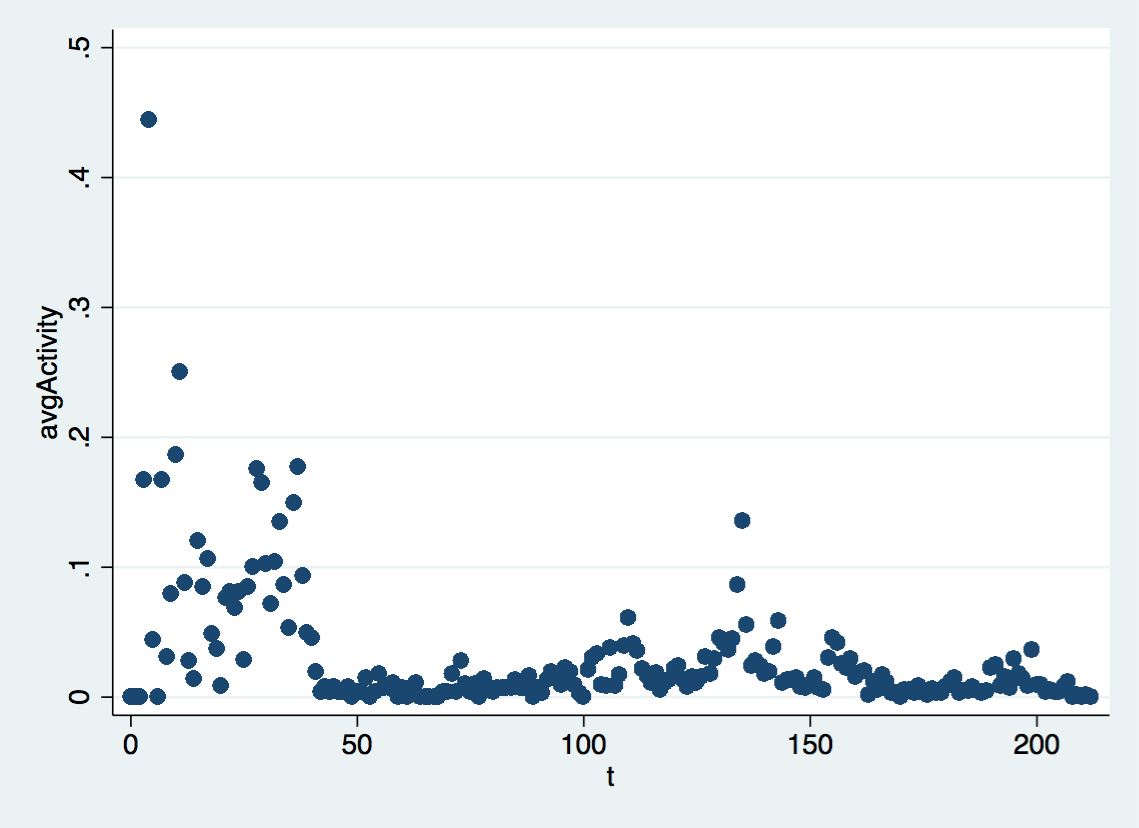
\includegraphics[width = \textwidth]{avgActivity_ER} 
	\caption{Average number of posts and comments written by non-community manager members of Edgeryders per week}
	\label{fig:avgActivityER}

\end{figure}

\section{Deciding who to engage with}

Next, community members who have decided to engage in communication events need to choose who to make the target of their communication. This is where the intimacy network plays an important role. The decision is modelled as follows:

\begin{equation}
	P [\phi_{ij}(t_n) = 1] = \frac{1 + \beta W_{ij}(t_{n-1}) W_{ji}(t_{n-1})}{\sum_j [1 + \beta W_{ij}(t_{n-1}) W_{ji}(t_{n-1})]}
	\label{eq:mainEngine}
 \end {equation}

The choice of who users communicate with is, in the model, a random choice according to a uniform distribution, influenced by the intimacy felt with each of the other users. The $\beta$ parameter represents intimacy strength: when it is set to 0, users communicate at random. The higher it gets, the more "conservative" users get in communicating almost always with people they are most intimate with. Note that, though $W_{i,j} \neq W_{j,i}$, the probability of a communication from $i$ to $j$ is identical to that of a communication from $j$ to $i$, that is $P [\Phi_{i,j}(t_n) = 1] = P [\Phi_{j,i}(t_n) = 1]$. This implies assuming that users prefer to address their communication either with people that talk to them more, and with people that they themselves talk more to. 

This part of the model is lifted straight from \cite{kim2015group}. 

\section{Updating the intimacy network}

Next, all pairwise intimacy values are updated as follows:

\begin{equation}
	W_{ij}(t_n) = W_{ij}(t_{n-1})e^{-\frac{\Delta t}{\tau}} + \Phi_{ij}(t_n)
	\label{eq:updating}
\end{equation}

Where $\tau$ is a time discount rate. This, too, is lifted from \cite{kim2015group}.

\section{New members join the community}

At the beginning of each period, we exogenously add $\alpha$ new members.

\section{Community managers}

At each period, community managers engage in activities expected to increase engagement and inclusivity in the online community. Community managers use the same platform as ordinary users, who do not always clearly distinguish between their fellow "ordinary" users and the "special" ones that work as community managers. We can therefore keep track of the activity of community managers by representing them as a special node in the intimacy network, whose behaviour follows rules dictated by the organisation running the online community.

\subsection{Onboarding}

Among professional online community managers, onboarding is the activity of welcoming a new user. Welcome messages often include some practical information. In this paper, we assume that welcome messages are addressed to all new users, regardless of whether they engage in communications or not. 

Under a policy of onboarding, all new users are made the target of a welcome message by community managers only one, in the period at which they join the network.  Equation \ref{eq:mainEngineOnboarding}  describes the behaviour of the community manager special user as she chooses who to interact with: 

\begin{equation}
	P [\phi_{cj}(t_n) = 1] = 
	\begin{cases}
		1, & \text{if}\ j \text{ joined at } \ t_{n-1} \\
		0, & \text{otherwise}
	\end{cases}
	\label{eq:mainEngineOnboarding}
\end{equation}

Where the index $c$ denotes the community manager, so that in $\phi_{cj}$ denotes the communication event from the community manager to user $j$.

\subsection{Engagement}

\textit{Engagement} is a community management policy that consists of replying to posts of community members, whether or not they are new to the community. Its rationale is to reward continued engagement of community members \footnote{This is relatively common in some online forums, for example in those associated to MOOCs, like Coursera's.}.  

Under a policy of engagement, a share $q$ of users that have been active at time $t_{n-1}$ receive a communication from community managers at time $t$. Equation \ref{eq:mainEngineEngagement}  describes the behaviour of the community manager special user as she chooses who to interact with: 

\begin{equation}
	P [\phi_{cj}(t_n) = 1] = 
	\begin{cases}
		q, & \text{if}\ \exists i \neq j : \phi_{ji}(t_{n-1}) =1 \\
		0, & \text{otherwise}
	\end{cases}
	\label{eq:mainEngineEngagement}
\end{equation}

\section{Research questions}

Kim, Jo and Kim use their model to show that online communities where intimacy plays an important role (i.e. where the parameter $\beta$ is high) are "exclusionary" towards newcomers. New members find it hard to integrate. Most eventually give up and disengage completely\footnote{They do so when their incoming intimacy is "too low". A threshold parameter is set exogenously to regulate this. The advantage of such a choice is that the authors can then study the effect of the value of $\beta$ on network topology. They go on to show that the network becomes more sparse as $\beta$ increases.

I think that "leaving the network" is not necessary. We are interested in the social attribute of "being fully included in the online community". In terms of the model, this can be approximated by incoming intimacy, i.e. weighted in-degree in the intimacy network, denoted in \cite{kim2015group} by $S$ (for "membership strength"). Removal from the network is represented by setting $S$ to zero when it drops below the threshold value. Kim, Jo and Kim could as well have ignored thresholds and looked at the distribution of $S$ across users as a proxy of community inclusivity. 

I advocate doing so, both for elegance reasons and because I question the metaphor. "Leaving" seems like an active choice to say farewell: this is very rare in real-world online communities, where users tend to become inactive gradually, until their perfectly valid accounts sit completely still. The only real-world online communities where the number of accounts decreases are those where the organisations running them have a policy of terminating inactive accounts after a certain time (Pardus), or if they fail to pay fees (World of Warcraft). 
}. 

Disengagement (or, more generally, low engagement) is clearly not desirable from the point of view of the organisation running the online community, because higher retention of new members and higher engagement map increase the value of the online community seen as an asset. However, the model specified here differs significantly from that of \cite{kim2015group}. So, we start by asking whether Kim, Jo and Kim's main result is robust to this new, more realistic model specification. 

\newtheorem{intimacy}{Hypothesis}

\begin{intimacy}
	Increasing the value of the intimacy parameter $\beta$ has no effect on the level of exclusion in the online community. 
	\label{intimacyModelHolds}
\end{intimacy}

To disprove, run the computer simulation with different values of $\beta$. Obtain and compare the distributions of membership strength corresponding to different values of $\beta$. We expect the alternative hypothesis to be true, with higher values of $\beta$ corresponding to higher levels of exclusion. 

\begin{intimacy}
	Onboarding by online community managers has no effect on the level of exclusion in the online community.
\end{intimacy}

To disprove, run the computer simulation with and without the special user representing the activity of online community manager. Obtain and compare the distributions of membership strength corresponding to each case. We expect the alternative hypothesis to be true, with a higher levels of exclusion corresponding to the absence of an onboarding policy. 

\begin{intimacy}
	Engagement by online community managers has no effect on the level of exclusion in the online community.
\end{intimacy}

To disprove,  run the computer simulation with different values of $q$. Obtain and compare the distributions of membership strength corresponding to different values of $q$. We expect the alternative hypothesis to be true, with higher values of $q$ corresponding to lower levels of exclusion. 

\section{Comparing distributions of membership strength}

All hypothesis testing is based on the idea of comparing distributions. This happens as follows:

\begin{itemize}
	\item Each run of the model generates a distribution of the membership strength value $S_i$ associated with each member $i$ of the online community. 
	\item We obtain one (or more) statistic from such distribution. The mean is not the most useful one, because we - like Kim, Jo and Kim - are interested in cliquishness and exclusion; the Gini coefficient could be a better fit, with a lower Gini coefficient indicating a more inclusive community.
	\item For each parameter vector, we run the model multiple times (100 times). Randomness in the model ensures that the distributions obtained will differ from each other. We therefore obtain a distribution of summary statistics (for example of Gini coefficients) for each parameter vector.
	\item The two distributions can then be compared, for example via a Kolmogorov-Smirnov test. 
\end{itemize}

\section{Parameter space and computational complexity}

The main parameters of this model are five. Three describe the online community without community managers intervention; the other two describe community management policies.

\begin{enumerate}
	\item "Chattiness" $C$.
	\item Responsiveness to incoming communication events $\delta$.
	\item Intimacy $\beta$.
	\item Onboarding. This is a binary condition, determined on whether equation \ref{eq:mainEngineOnboarding} is included or not in the model.
	\item Engagement intensity $q$.
\end{enumerate}

To a first approximation, exploring the parameter space would entail covering all combinations of the following cases.

\begin{enumerate}
	\item $C$ "low" and "high".
	\item $\delta$ "low" and "high"\footnote{Where "low" could correspond to $\delta = 0,015$ and "high" to $\delta = 0.2$, consistently with \cite{cottica2016microfoundations}.}.
	\item $\beta$ "low", "middle" and "high" (consistently with \cite{kim2015group}).
	\item Onboarding "off" or "on".
	\item $q$ "low" or "high". $q =0$ accounts for the absence of engagement policy.
\end{enumerate}

For each of these, we run the simulation at least 100 times, obtaining a distribution of distributions of membership strength $S_i$ for each point of the parameter space. We then reduce each distribution to one scalar indicator of inequality, and obtain a distribution of values of that indicator for each point in the parameter space. We then proceed to test that these distributions are drawn from the same population with the following algorithm:

\begin{enumerate}
	\item fix the values of the parameters describing the behaviour of the unmanaged community: $C = C^*, \delta = \delta^*, \beta = \beta^*$. 
	\item Compute the distribution of $S_i$ under this set of parameters and the following cases: 
	\begin{enumerate}[label*=\arabic*.]
		\item Onboarding "off", $q = 0$ (baseline, with no community management).
		\item Onboarding "on", $q = 0$ (only onboarding). 
		\item Onboarding "off", $q$ "low" and onboarding "off", $q$ "high" (only engagement).
		\item Onboarding "on", $q$ "low" and onboarding "on", $q$ "high" (both onboarding and engagement).
	\end{enumerate}
	\item Run tests comparing the baseline with the five possible community management policy combination.  
\end{enumerate}

There are eight possible combinations of $C$, $\delta$ and $\beta$. So, the study involves running 40 tests. The computer simulation as such is unlikely to be computationally expensive. The overall computational load of the paper depends on the statistical technique used to test the membership strength distributions against each other. If the latter are as simple as chi-square or Kolmogorov-Smirnov tests, the whole study can be conducted off a single computer.

	\bibliographystyle{plain}
	\bibliography{Engineering_inclusivity}
	
\end{document}